\documentclass{article}

\usepackage[T1]{fontenc}
\usepackage{graphicx}
\usepackage{fancyhdr}
\pagestyle{fancy}
\fancyhf{}
\lhead{Draft 0.1}
\rhead{Elliot Oram}
\rfoot{\thepage}


\title{Overall System Use Case}
\author{elo9@aber.ac.uk}

\begin{document}

\maketitle
\tableofcontents

\newpage

\section{Use Case diagram}
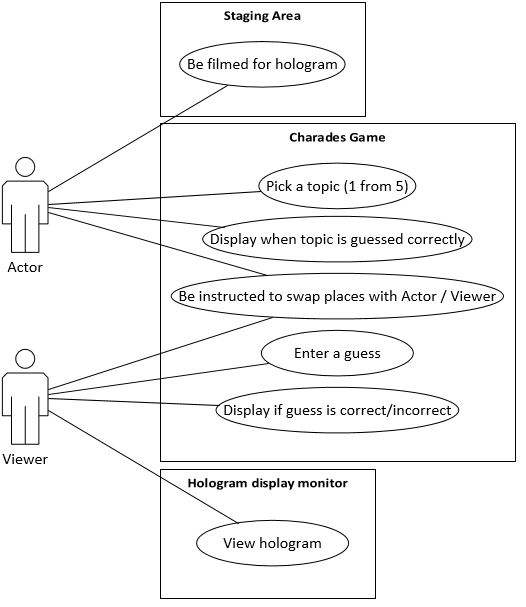
\includegraphics[width=\textwidth]{UseCaseImage}

\newpage


\section{Description of Use Cases}
\begin{enumerate}
	\item \textbf{Be filmed for hologram}: This action takes place in the staging area and refers to the ability for an Actor to be filmed. This does should not require any user input.
	
	\item \textbf{Pick a topic (1 from 5)}: This functionality is specific to the Charades Game and is the initial stage where the Actor selects the topic they wish to act out from 5 random topics displayed to them. The topics will be displayed via a tablet or small monitor mounted in the staging area.
	
	\item \textbf{Display when guess viewer guesses correctly}: This use case is where the system alerts the Actor that one of the viewers has guessed their topic correctly. This message will be displayed via the monitor in the staging area
	
	\item \textbf{Be instructed to swap places with Actor / Viewer}: Alert the Viewer, who successfully guessed the topic, and the Actor to switch places. Messages will be displayed in the staging area and on the device that correctly guessed the topic.
	
	\item \textbf{Enter a guess}: Use case allowing a Viewer to enter a guess (string) for the topic being acted out in the staging area. This will be displayed to a device that near the hologram (a tablet or addition monitor)
	
	\item \textbf{Display if guess was correct/incorrect}: Display to the if a guess was correct or incorrect. This action will feed into the 4th action listed above.
	
	\item \textbf{View hologram}: Viewers should be able to view the hologram from that is displayed on the monitor. This will also require the pyramid to be in place on the monitor.
\end{enumerate}

\section{Use cases for prototype}
In the case of the prototype, only use cases in the \textit{Hologram display monitor} and \textit{Staging Area} subsystems are required. There will be several features mentioned in the feature list that will reference these subsystems. 
Other use cases, mentioned under the \textit{Charades Game} subsystem will be required for the extension of the project after 

\end{document}